% !TEX program = lualatex
% region %%%%%%% document class & geometry %%%%%%%%%%%
\documentclass[12pt,a4paper]{article}
\usepackage[%
  top=2.5cm,
  bottom=2.5cm,
  left=2.5cm,
  right=2.5cm
]{geometry}
% endregion ==================

% region core packages %%%%%%%%%%%
\usepackage{%
  tikz,
  authblk,
  graphicx,
  lineno,
  csquotes,% loaded after lineno to avoid warning
  microtype,
  subcaption,% provides the subcaptionblock (subfigure) env.
  tabularray,
  siunitx,% for proper typesetting of units
  xcolor,% to define custom color
}
\usepackage[section]{placeins}% ensures figures stays in their sections
\usepackage[version=4]{mhchem}% typeset chemical formulas
% endregion ==================

\usepackage{kantlipsum}% for dummy text!

\date{}% do not print date

% define fonts
\usepackage{cochineal}

\graphicspath{{./img/}}% path for images

\UseTblrLibrary{booktabs}% for nicer-looking tables

\sisetup{mode=match}% print units in same font as surrounding text

\renewcommand{\thesubfigure}{% format of fig refs in legends
  \sffamily
  \textbf{(\Alph{subfigure})}
}

% region disable line numbers for section titles
\makeatletter
\patchcmd{\@startsection}{\@ifstar}{\nolinenumbers\@ifstar}{}{}
\patchcmd{\@xsect}{\ignorespaces}{\linenumbers\ignorespaces}{}{}
\makeatother
% endregion

% region comment large portion of text
\newbool{hideswitch}% boolean for commented code
\booltrue{hideswitch}% ignore commented code by default
%\boolfalse{hideswitch}% uncomment this line to print out/run commented text
\newcommand{\hide}[1]{%
  \ifbool{hideswitch}
    {}% output nothing if boolean true
    {#1\ignorespaces}% else print out/run comment
}
% endregion% other custom settings and commands
% region fix superscript for authblk package
\makeatletter
\renewcommand\AB@authnote[1]{{\normalfont\textsuperscript{#1}}}
\renewcommand\AB@affilnote[1]{{\normalfont\textsuperscript{#1}}}
\makeatother
% endregion fix superscript ====
\title{Informative title proves to be helpful to unsuspecting reader}
\author[1,*]{Immanual Kant}
\author[1]{Michael Clouscard}
\author[1, 2]{György Lokács}
\affil[1]{Department of Philosophy, University of Milan}
\affil[2]{Department of Biology, Polish Institute of Sciences}
\affil[*]{correspondance: ikant@help.it}
\usepackage[%
  backend=biber,
  style=authoryear,
  uniquename=init,
  giveninits=true,
  doi=false,
  isbn=false,
  eprint=false,
  url=false,
  date=year,
  sorting=ydnt,
  maxcitenames=1,
  mincitenames=1,
  maxbibnames=12,
  minbibnames=2,
]{biblatex}

\addbibresource{references.bib}
\renewcommand*{\bibfont}{\small}% define biblio font
\renewbibmacro{in:}{}% remove "in" before journal
\DeclareFieldFormat{labelnumberwidth}{#1.\space}% remove square brackets in biblio
\DeclareFieldFormat{journaltitle}{#1\isdot}% ensure journal name is upright

\DefineBibliographyStrings{english}{% make et al in italic
  andothers = {\mkbibemph{et\addabbrvspace al\adddot}}}
% remove comma before "et al"
\DefineBibliographyExtras{english}{%
  \let\finalandcomma=\empty
  \let\finalandsemicolon=\empty
}

\AtEveryBibitem{%
  \clearfield{volume}% remove vol. number
  \clearfield{number}% remove issue number
}% biblatex settings

%%%%%%%%%% document body %%%%%%%%%%%
\begin{document}
\maketitle
\begin{abstract}
This is a simple, generic template which is designed to be functional.
Most journals do not accept \LaTeX{} documents, and the ones who do will modify the typesetting so there is no much point in making a fancy template.
\end{abstract}

keywords: reality, frustration, debugging% contains keywords

\linenumbers
\section{Introduction}
\hide{
  This text is not displayed.
  Visibility is under the control of \texttt{hideswitch} defined in the \texttt{custom} file.
}
This is a sentence with some citations at the end \parencite{ramachandran2021,saito2018}.
The following is some text by Kant: \kant[3]
\section{Materials and Methods}
\subsection{Plant materials and growth conditions}
All experiments were performed on tomato (\textit{ Solanum lycopersicum}) grown in rockwool supplemented with a \={O}tsuka house 1 and 2 (OAT Agrio Co., Ltd, Japan) nutrient solution under a 16-hour light/8-hour dark regime under LED lights outputting \SI{230}{\micro\mole\per\square\meter\per\second} of PAR.

\subsection{Microscopy}
We used a \qty{0.05}{\percent} toluidine blue for staining.

\subsection{Bioinformatics analysis}
We performed a blastp (protein-protein BLAST) with default parameters using the National Center for Biotechnology Information (NCBI; https://blast.ncbi.nlm.nih.gov/Blast.cgi) database on the non-redundant protein sequences (nr) data subset.
\section{Results}
\kant[6]

\begin{table}[h]% placement enforced with [h]
  \begin{center}
    \begin{tblr}{
      colspec={Q[l] Q[l] Q[l]},
      rowsep=0.15\baselineskip,
    }
      line & value & cuteness \\
      \hline
      WT      & 25     & moderate             \\
      double-cat  & 40     & high          \\
      \hline
    \end{tblr}
  \end{center}
\caption{A WT single cat scored 25, significantly less than a double-cat.}
\label{table:cuteness_index}
\end{table}

\kant[7]
\begin{figure}
  \centering
  \sffamily % font family for labels (does not include legend)
  % subfigure A
  \begin{tikzpicture}
    \node[anchor=north west] at (-1em, 0em) {% label
      \textbf{A}
    };
    \node[anchor=north west] at (0em, 0em) {% image
      \begin{subcaptionblock}{0.25\textwidth}
        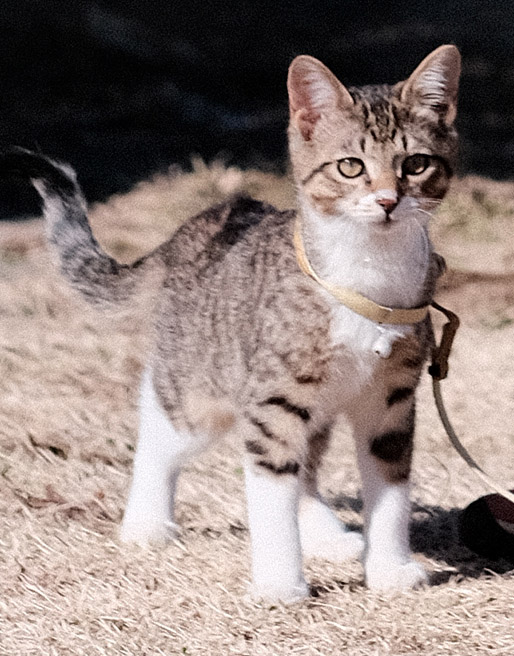
\includegraphics[width=\textwidth]{one_cat.jpg}
        \phantomcaption\label{cat}
      \end{subcaptionblock}
    };
    \node[% inner label
      anchor=north west,
      fill=white,
      fill opacity=0.8,
      text opacity=1,
      inner sep=0.2em
    ] at (1ex, -1ex) {WT};
  \end{tikzpicture}
  \hfill
  % subfigure B
  \begin{tikzpicture}
    \node[anchor=north west] at (-1em, 0em) {
      \textbf{B}
    };
    \node[anchor=north west] at (0em, 0em) {
      \begin{subcaptionblock}{0.62\textwidth}
        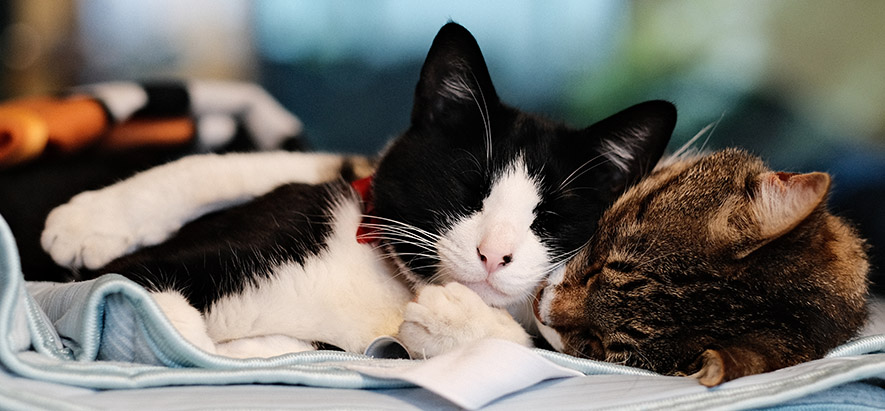
\includegraphics[width=\textwidth]{two_cats.jpg}
        \phantomcaption\label{twocats}
      \end{subcaptionblock}
    };
  \end{tikzpicture}
  % main caption
  \caption{Some cats.
   In \subref{cat}, a single cat being cute.
   \subref{twocats} shows increased cuteness associated with a higher number of cats.}
  \label{fig:cats}
\end{figure}
See figure~\ref{fig:cats} to see some cat pictures.
More data about these cats can be found in table~\ref{table:cuteness_index}.
\section{Discussion}
\kant[10]

\subsection*{Author contributions}
Conceptualization, X.X. and Y.Y.; methodology, X.X.; software, X.X.; validation, X.X., Y.Y. and Z.Z.; formal analysis, X.X.; investigation, X.X.; resources, X.X.; data curation, X.X.; writing---original draft preparation, X.X.; writing---review and editing, X.X.; visualization, X.X.; supervision, X.X.; project administration, X.X.; funding acquisition, Y.Y. All authors have read and agreed to the published version of the manuscript.

\subsection*{Funding}
This research was funded by NAME OF FUNDER grant number XXX.

\subsection*{Acknowledgments}
We acknowledge technical support, donations, etc.

\subsection*{Conflicts of interest} The authors declare no conflict of interest.
\printbibliography
\end{document}